\documentclass[a4paper,8pt]{report}
\setcounter{tocdepth}{3}

\usepackage[utf8]{inputenc}
\usepackage[latin1]{inputenc}
\usepackage[francais]{babel}
%\usepackage[T1]{fontenc}

\usepackage[left=2cm]{geometry}
\usepackage{amsmath,amssymb,mathrsfs}
\usepackage{graphicx}
\usepackage[table,xcdraw]{xcolor}

\usepackage{enumerate}

\usepackage{pgfplots}
\usetikzlibrary{shapes,positioning}
\usepackage{tikz}

\usepackage[nottoc, notlof, notlot]{tocbibind}
\usepackage{verbatim}

\usepackage{bibentry}

\usepackage{fullpage}

%\tikzset{state/.style={circle,draw=black, very thick,minimum size=4em}}

%Utilisation des codes sources en C
\usepackage{listings}
\lstset{
  language=C,
  language=Bash,
  basicstyle=\footnotesize,
  numbers=left,
  numberstyle=\normalsize,
  numbersep=7pt,
}

\begin{document}

\begin{titlepage}
\newcommand{\HRule}{\rule{\linewidth}{0.5mm}} % Defines a new command for the horizontal lines, change thickness here
\center % Center everything on the page
 
%----------------------------------------------------------------------------------------
%HEADING SECTIONS
%----------------------------------------------------------------------------------------

\textsc{\LARGE Universit\'e Pierre et Marie Curie}\\[1.5cm] % Name of your university/college
\textsc{\Large Projet SAR}\\[0.5cm] % Major heading such as course name
%\textsc{\large Minor Heading}\\[0.5cm] % Minor heading such as course title

%----------------------------------------------------------------------------------------
%TITLE SECTION
%----------------------------------------------------------------------------------------

\HRule \\[0.4cm]
{ \Huge \bfseries Kilobot}\\[0.4cm] % Title of your document
Impl\'ementation d'algorithmes pour les cohortes de robots
\HRule \\[1.5cm]
 
%----------------------------------------------------------------------------------------
%AUTHOR SECTION
%----------------------------------------------------------------------------------------

\begin{minipage}{0.4\textwidth}
\begin{flushleft} \large
\emph{Auteurs:}\\
Arnaud \textsc{Guermont} % Your name
\\Benjamin \textsc{Bielle} % Your name
\end{flushleft}
\end{minipage}
~
\begin{minipage}{0.4\textwidth}
\begin{flushright} \large
\emph{Superviseur:} \\
Dr. Swan \textsc{Dubois} % Supervisor's Name
\end{flushright}
\end{minipage}\\[4cm]

% If you don't want a supervisor, uncomment the two lines below and remove the section above
%\Large \emph{Author:}\\
%John \textsc{Smith}\\[3cm] % Your name

%----------------------------------------------------------------------------------------
%DATE SECTION
%----------------------------------------------------------------------------------------

{\large \today}\\[3cm] % Date, change the \today to a set date if you want to be precise

%----------------------------------------------------------------------------------------
%LOGO SECTION
%----------------------------------------------------------------------------------------

%
\includegraphics[width=4cm]{images/upmc.png}\\[1cm] % Include a department/university logo - this will require the graphicx package
 
%----------------------------------------------------------------------------------------

\vfill % Fill the rest of the page with whitespace

\includegraphics[width=4cm]{images/upmc.png}\\[1cm] % Include a department/university logo - this will require the graphicx package
\end{titlepage}

\renewcommand{\contentsname}{Sommaire}
\tableofcontents
\listoffigures

%%%%%%%%%%%%%%%%%%%%%%%%%%%%%%%%%%%%%%%%%%%%%%%%%%%%%%%%%%%%%%%%%%
%                                                                %
%                          INTRODUCTION                          %
%                                                                %
%%%%%%%%%%%%%%%%%%%%%%%%%%%%%%%%%%%%%%%%%%%%%%%%%%%%%%%%%%%%%%%%%%
\chapter{Introduction}

%\noindent \textbf{Ma\^itrise d'oeuvre :} DUBOIS Swan.\\
%\noindent \textbf{Ma\^itrise d'ouvrage :} GUERMONT Arnaud, BIELLE Benjamin.\\

\section*{Contexte}\label{sec:name}
\addcontentsline{toc}{section}{Contexte}

\textbf{Kilobot} est une plate-forme constitu\'ee de petits robots autonomes. Cette plate-forme est propos\'ee par l'universit\'e d'Harvard\footnote{http://www.eecs.harvard.edu/ssr/projects/progSA/kilobot.html}. \\
Ces robots se d\'eplacent uniquement par vibration et communiquent par infrarouges.\\

\begin{figure}[!h]
    \centering
    \subfigure{ 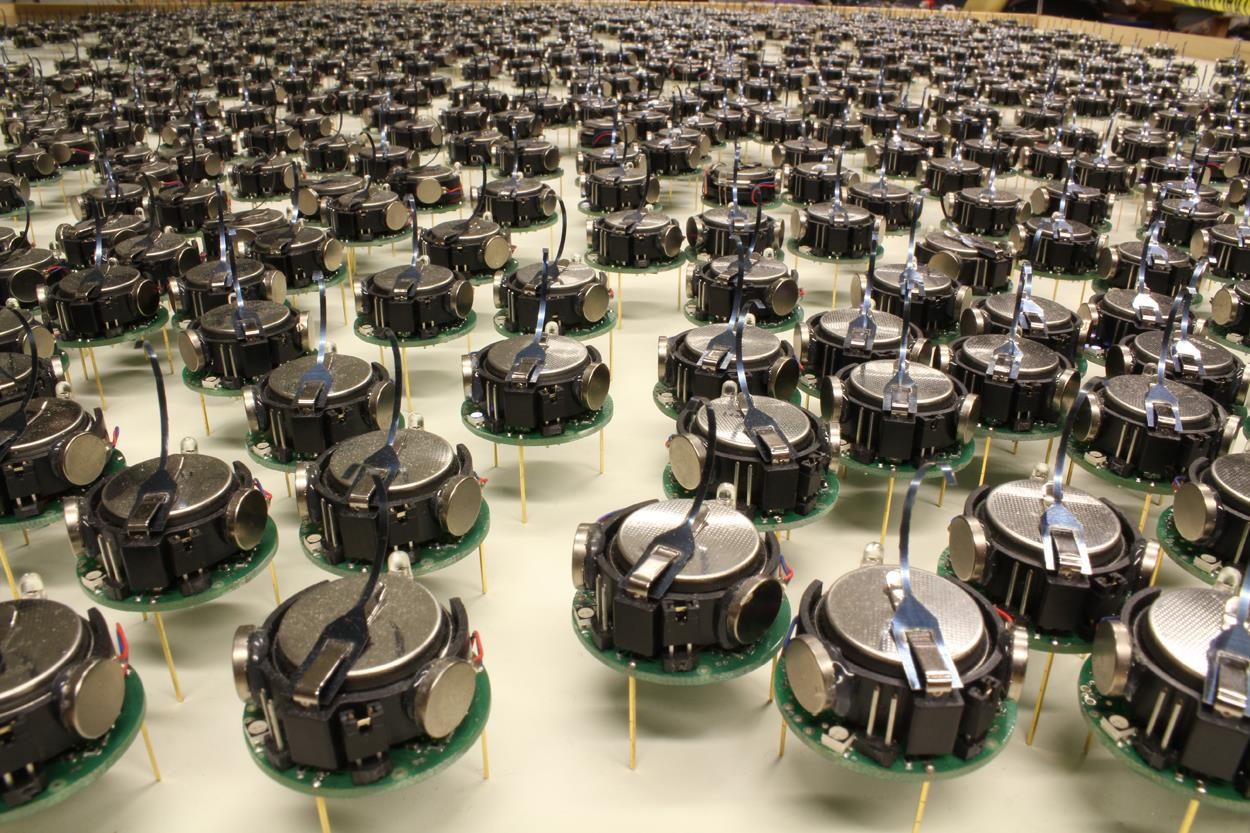
\includegraphics[width=6cm]{images/kilobotI.jpg}}
    \subfigure{ 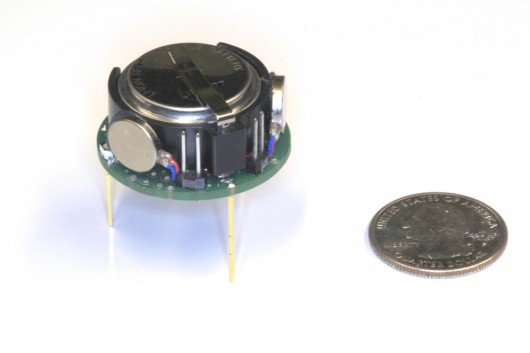
\includegraphics[width=6cm]{images/kilobotII.jpg}}
    \caption{Robots Kilobot}
\end{figure}

\smallskip
Le projet a pour objectif d'impl\'ementer des algorithmes r\'epartis sur un essaim de robots (la plate-forme \textbf{Kilobot}).\\
Il se d\'ecoupe en trois phases, la premi\`ere consiste en une recherche documentaire et une prise en main de la plate-forme mat\'erielle, la seconde concerne l'impl\'ementation d'algorithmes (dans notre cas de bio-algorithmes). Enfin la derni\`ere phase se concentre sur la recherche des possibilit\'es d'impl\'ementation d'un mod\`ele : le \textbf{mod\`ele CORDA}\footnote{Giuseppe Prencipe. A new distributed model to control and coordinate a set of autonomous mobile robots : The corda model, 2000.}.\\

%Le but de ce projet est d'impl\'ementer une \textbf{API} permettant de manipuler des mod\`eles robotiques sur la plate-forme Kilobot. Ces mod\`eles ne sont pas pr\'evus pour la plate-forme Kilobot, notre API devra rendre cette impl\'ementation possible en restant simple et si possible facilement extensible.\\

\bigskip

\section*{L'existant}\label{sec:name}
\addcontentsline{toc}{section}{L'existant}

Il existe deux API de base pour la plate-forme Kilobot :\\

\begin{itemize}
\item \textit{\textbf{K-team}}\footnote{http://www.k-team.com/mobile-robotics-products/kilobot}.
\item \textit{\textbf{Kilobotics}}\footnote{https://www.kilobotics.com/}.
\end{itemize}

\medskip
Celle propos\'ee par \textit{\textbf{K-team}} (fournie par d\'efaut avec les robots) nous permet une moins grande libert\'e que celle de \textit{\textbf{Kilobotics}}.\\
Donc notre \textit{\textbf{API}} se basera sur celle-ci car elle nous garantit une plus grande libert\'e, portabilit\'e et extensibilit\'e.

\section*{Veille Technologique}\label{sec:name}
\addcontentsline{toc}{section}{Veille Technologique}

Il existe plusieurs projets similaires aux kilobots, par exemple le projet \textit{\textbf{I-Swarm}}\footnote{http://www.hizook.com/blog/2009/08/29/i-swarm-micro-robots-realized-impressive-full-system-integration} (trop limités techniquement), mais seule la plate-forme \textit{\textbf{Kilobot}} permet de manipuler des centaines de robots de mani\`ere r\'ealiste hors d'un simulateur (avec un prix convenable).\\
Le projet \textit{\textbf{E-Swarm}}\footnote{http://www.e-swarm.org/research_main.php} propose une plate-forme int\'eressante mais le prix de chaque robot en fait une plate-forme non \'eligible pour ce projet.\\

\begin{figure}[!h]
    \centering
    \subfigure{ 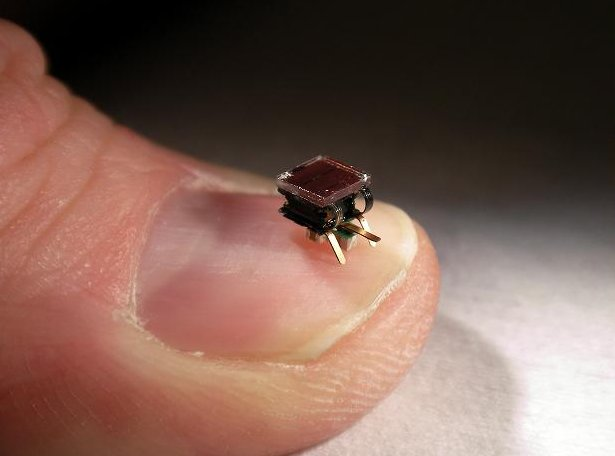
\includegraphics[width=7cm]{images/iSwarm.jpg}}
    \subfigure{ 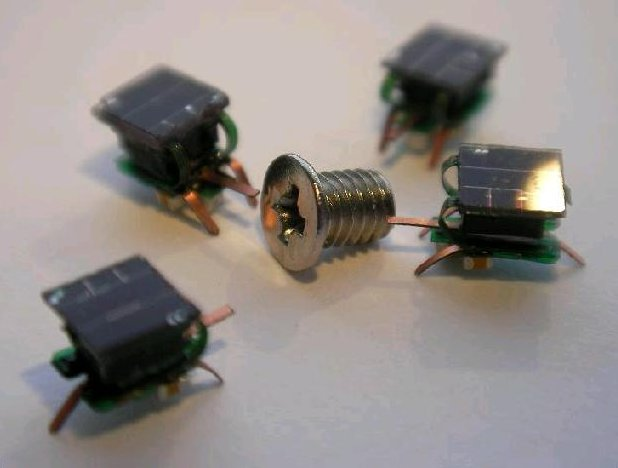
\includegraphics[width=7cm]{images/iSwarmII.jpg}}
    \caption{Robots I-Swarm}
\end{figure}

\begin{figure}[!h]
    \centering
    \subfigure{ 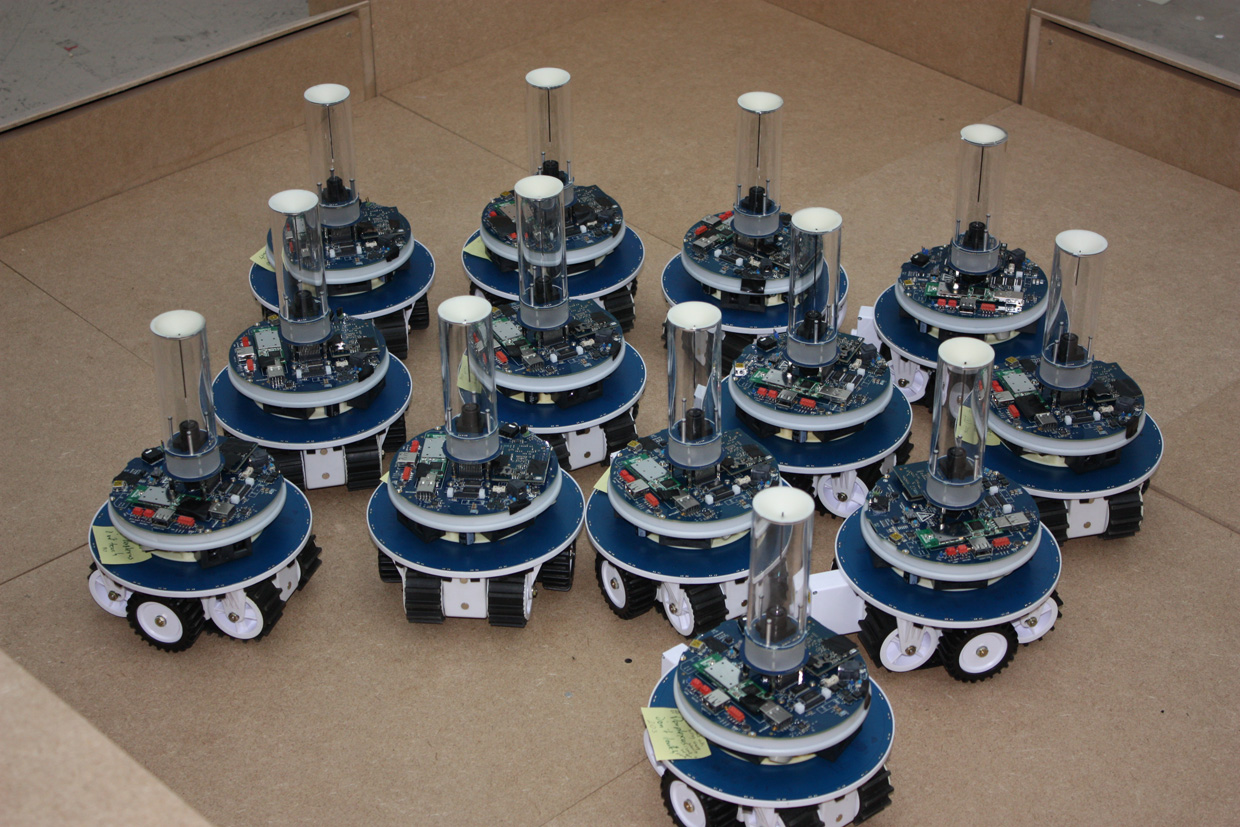
\includegraphics[width=8cm]{images/eSwarmII.jpg}}
    \subfigure{ 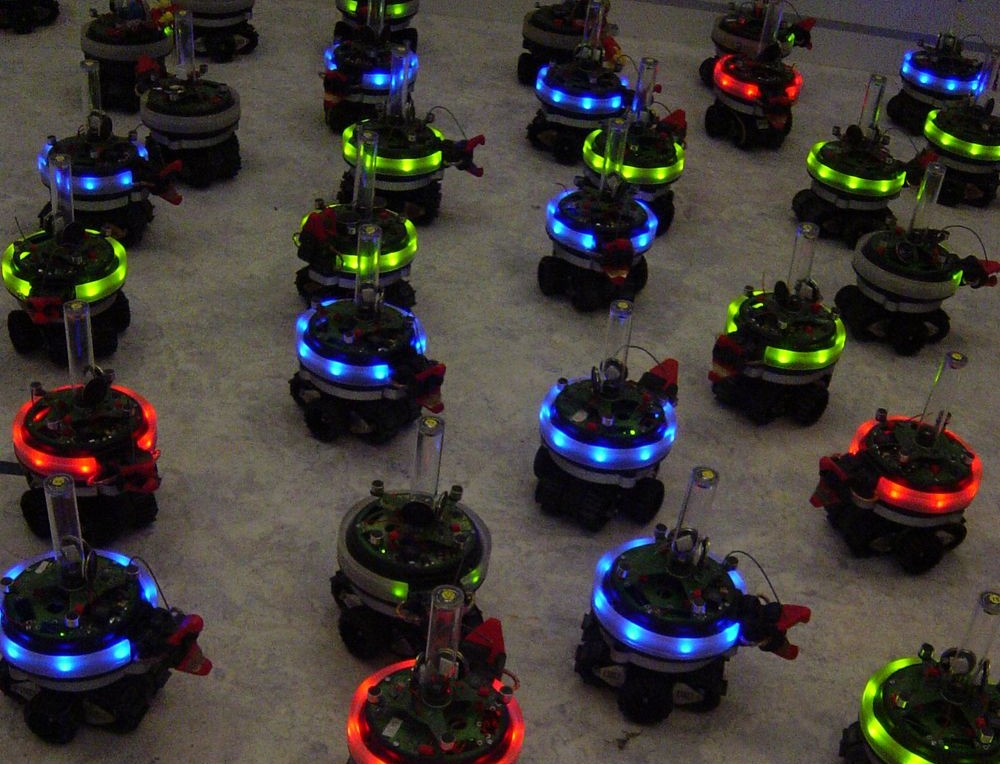
\includegraphics[width=7cm]{images/eSwarmIII.jpg}}
    \caption{Robots E-Swarm}
\end{figure}

%%%%%%%%%%%%%%%%%%%%%%%%%%%%%%%%%%%%%%%%%%%%%%%%%%%%%%%%%%%%%%%%%%
%                                                                %
%                          SPECIFICATIONS                        %
%                                                                %
%%%%%%%%%%%%%%%%%%%%%%%%%%%%%%%%%%%%%%%%%%%%%%%%%%%%%%%%%%%%%%%%%%
\chapter{Sp\'ecifications}

\section*{Mat\'erielles}\label{sec:name}
\addcontentsline{toc}{section}{Mat\'erielles}

Le but du mod\`ele est de repr\'esenter une grande quantit\'e de robots (presque un essaim) pour pouvoir effectuer des t\^aches collectives qui seraient impossibles \`a r\'ealiser en solitaire. De nombreux exemples dans la nature mettent en action ce principe : les fourmis peuvent explorer des zones d'un p\'erim\`etre de plusieurs kilom\`etres par exemple. \\
Dans la robotique, il existe des algorithmes divers telle-que l'auto-assemblage, les constructions collectives ou encore l'exploration.\\ 
Ces algorithmes sont faits pour \^etre test\'es sur plusieurs centaines voir milliers d'individus. Cependant, pour des raisons de co\^uts, de temps ou encore de complexit\'e, il est parfois uniquement possible de les valider en simulation. \\
C'est pourquoi un mod\`ele comme celui que les kilobots impl\'ementent fut cr\'e\'e. Les robots devaient avoir plusieurs capacit\'es : communiquer et percevoir leur environnement par l'interm\'ediaire de capteurs, conna\^itre la distance entre eux et se d\'eplacer en avant, tourner sur la gauche et sur la droite. De plus, ils devaient aussi pouvoir tous \^etre contr\^ol\'es ensemble simultan\'ement par un seul op\'erateur. Mais la principale contrainte restait le co\^ut. En effet, il \'etait tr\`es dur auparavant de tester des algorithmes sur des essaims de robots qui co\^utaient plusieurs centaines de dollars \`a l'unit\'e.\\

\subsection*{Communication et perception de l'environnement}\label{subsec:name}
\addcontentsline{toc}{subsection}{Communication et perception de l'environnement}

De nombreux algorithmes collectifs utilisent la communication entre robots et la distance entre ces m\^eme robots pour piloter individuellement le comportement de chaque robot. Il est donc indispensable que les kilobots puissent communiquer entre eux ainsi que mesurer la distance qui les s\'epare l'un de l'autre. \\
Pour qu'ils puissent communiquer, chaque kilobot est pourvu d'une led pour transmettre et d'une photodiode infrarouge comme r\'ecepteur qui sont toutes les deux plac\'ees en-dessous au centre du robot. En \'etant plac\'e au centre, le r\'ecepteur peut recevoir des messages d'une \'egale distance dans toutes les directions. Les messages sont envoy\'es par la led et utilisent la r\'eflexion du support sur lequel ils \'evoluent pour transmettre (c'est pourquoi le support doit \^etre r\'efl\'echissant comme un tableau blanc ou un miroir par exemple). En utilisant cette technique, un kilobot peut transmettre dans un rayon de 7 centim\`etres \`a un d\'ebit de 30 kb/s. La m\'ethode d'acc\`es CSMA/CA est utilis\'ee pour \'eviter les collisions (tous les robots \'emettent sur le m\^eme canal).\\
Une led RGB est aussi situ\'ee sur le c\^ot\'e pour pouvoir informer l'utilisateur.\\

\medskip
Les kilobots sont aussi pourvus d'un capteur de lumi\`ere permettant de mesurer l'intensit\'e lumineuse de l'environnement du robot.\\

\subsection*{Mesure de la distance}\label{subsec:name}
\addcontentsline{toc}{subsection}{Mesure de la distance}

Le calcul de la distance entre un robot et un autre se fait via l'envoi et la r\'eception du message. L'intensit\'e de la lumi\`ere \'emise par la led diminue proportionnellement avec la distance qu'elle parcourt. Il ne reste alors plus qu'au r\'ecepteur \`a calculer la distance en fonction de l'intensit\'e du signal re\c cu. Comme le signal peut \^etre affect\'e par l'environnement, la pr\'ecision est de +/- 2 mm.\\

\subsection*{D\'eplacement}\label{subsec:name}
\addcontentsline{toc}{subsection}{D\'eplacement}

L'une des principales capacit\'es des robots est de pouvoir se mouvoir dans leur environnement. L'une des solutions les plus simples et efficaces est d'utiliser un design \`a deux roues, chaque roue \'etant contr\^ol\'ee par un moteur. Mais cette solution est aussi tr\`es ch\`ere et ne permettra pas de r\'ealiser un robot \`a bas co\^uts. \\
Pour y rem\'edier, les kilobots disposent de trois jambes rigides et de deux moteurs \`a vibration dispos\'es de chaque c\^ot\'e du robot. Lorsqu'un des moteurs est activ\'e, il g\'en\`ere une force centrip\`ete qui est convertie en une force vers l'avant transmise \`a la jambe situ\'e en dessous du moteur. Gr\^ace au positionnement d\'ecentr\'e de chaque moteur, la mise en marche de l'un ou l'autre va causer une rotation vers la gauche ou la droite en fonction du moteur. En activant les deux moteurs en m\^eme temps et en contr\^olant la magnitude de leur vibration, ils est alors possible de faire avancer le robot en ligne droite vers l'avant. Il peut ainsi se d\'eplacer \`a une vitesse d'environ 1 cm/s et pivoter \`a environ 45\degre/s.\\

\subsection*{Contr\^ole des robots par l'op\'erateur}\label{subsec:name}
\addcontentsline{toc}{subsection}{Contr\^ole des robots par l'op\'erateur}

Lorsqu'on utilise un tr\`es grand nombre de robots, le chargement de leur programme, leur mise en marche ou encore le rechargement de leur alimentation peut vite prendre beaucoup de temps pour l'utilisateur : \'emettons l'hypoth\`ese qu'il faille 3 secondes pour allumer un robot via un interrupteur. Pour un groupe de 1000 robots, cela prendrait au total 50 minutes, ce qui est bien trop long pour \^etre efficace. \\
Les kilobots sont donc con\c cus pour \^etre utilis\'es \`a grande \'echelle par une seule personne.\\

\medskip
La communication entre l'op\'erateur et les robots passe par un contr\^oleur. Le contr\^oleur est une plate-forme disposant d'une connexion usb pour interagir avec l'ordinateur de l'utilisateur et de multiples led pour envoyer des messages aux kilobots. Chaque kilobot dispose sur son dos d'un r\'ecepteur pour la r\'eception des signaux. Le contr\^oleur est l'interface entre l'op\'erateur et l'essaim de robots. Dispos\'e \`a une hauteur d'un m\`etre, il couvre un p\'erim\`etre d'un m\`etre. Il permet d'effectuer de multiples op\'erations comme la mise en veille, le r\'eveil, le chargement d'un nouveau programme ou encore l'arr\^et du programme en cours d'ex\'ecution. Il est aussi utilis\'e pour la calibration des moteurs des kilobots.\\

\medskip
Le probl\`eme \'evoqu\'e auparavant aurait aussi pu s'appliquer aux kilobots. Pour y rem\'edier, les robots disposent d'un mode veille. Le microcontr\^oleur peut d\'esactiver le r\'egulateur de tension pour les moteurs et aussi celui pour le syst\`eme de communication (led et r\'ecepteur). Il ne reste plus que celui pour le microcontr\^oleur principal. Dans cet \'etat de veille, le microcontr\^oleur va tester toutes les minutes pendant 10 ms s'il a re\c cu un message de r\'eveil. Si c'est le cas, il r\'ealimente alors les r\'egulateurs de tension et le robot redevient de nouveau op\'erationnel. Ce mode veille permet \`a un kilobot d'avoir une autonomie de 3 mois. Mettre en veille un groupe ne prend que quelques secondes et le r\'eveil s'effectue en moins d'une minute. Les kilobots disposent aussi d'un interrupteur coupant toute alimentation du robot si ces derniers venaient \`a ne pas \^etre utilis\'es pendant une longue p\'eriode.\\

\medskip
Le rechargement de l'alimentation des robots est aussi un facteur de temps. Les kilobots disposent d'une batterie au lithium-ion de 3.4 V 160 mAh. Elle leurs assure une autonomie entre 3 et 24 heures selon l'usage qui en est fait. Le rechargement de celle-ci est aussi adapt\'e \`a la manipulation d'un grand nombre de robots. Pour cela, les kilobots utilisent deux de leurs trois jambes comme conducteur : l'utilisateur place les jambes des robots en contact avec un courant \'electrique de 6V via une plaque m\'etallique ou un tube m\'etallique et connecte le crochet situ\'e sur le dessus du robot \`a la masse. Cela permet le rechargement de plusieurs kilobots simultan\'ement sans intervention sur le robot. Par exemple, l'utilisation d'une plaque m\'etallique comme chargeur et d'une autre plaque qui viendrait se poser au dessus des kilobots est une solution abordable et adaptable \`a tr\`es grande \'echelle. Lorsque le chargement est termin\'e, la led RGB des kilobots en informe l'utilisateur.\\

\medskip
Le chargement d'un programme s'effectue via le contr\^oleur. Lorsque l'op\'erateur souhaite charger un nouveau programme, il envoie un message aux kilobots pour qu'ils placent leur pointeur de programme dans le bootloader. Ce dernier dispose d'un programme qui va alors recevoir le nouveau programme de l'utilisateur et le placer dans la m\'emoire primaire. Le bootloader va ensuite v\'erifier que ce programme ne dispose pas d'erreur puis ensuite red\'emarrer le kilobot qui va alors ex\'ecuter le nouveau programme. Cette m\'ethode permet de programmer un essaim de robots en environs 35 secondes. \\

\subsection*{Co\^uts}\label{subsec:name}
\addcontentsline{toc}{subsection}{Co\^uts}

La principale contrainte lorsqu'on impl\'emente un mod\`ele \`a large \'echelle est le co\^ut. En effet, les robots actuels d\'epassent les centaines de dollars \`a l'unit\'e et ne sont donc pas envisageables. \\
Les kilobots ont \'et\'e con\c cus dans le but de ne pas \^etre ch\`eres \`a construire. Le co\^ut \`a l'unit\'e pour 1000 robots est de 14 dollars, ce qui est environ dix fois moins que les autres robots con\c cus pour les algorithmes collectifs. \\
Pour cela, les robots disposent d'un moyen de locomotion par vibration comme vu auparavant et sont constitu\'es de pi\`eces simples et peut co\^uteuses : \\

\begin{itemize}
\item D\'eplacement : 3,12 \$
\item Alimentation : 3,61 \$
\item Communication/Capteur : 2,20 \$
\item Contr\^oleur : 2,83 \$
\item Structure : 1,55 \$
\item Divers : 0,74 \$
\item Total : 14,05 \$
\end{itemize}

\medskip
L'assemblage des robots est aussi tr\`es simple et rapide (la plupart des composants sont mont\'es \`a la  surface du PCB) et peut \^etre r\'ealis\'e par un robot pour un co\^ut d'environ 5 \$ par robot (pour 1000 robots). Cela prend donc environ 5 minutes pour obtenir un robot fonctionnel \`a partir des composants.\\

\section*{Logicielles}\label{sec:name}
\addcontentsline{toc}{section}{Logicielles}

\subsection*{Simulation}\label{subsec:name}
\addcontentsline{toc}{subsection}{Simulation}

Lorsqu'on impl\'emente des algorithmes collectifs, on d\'esire parfois les simuler avant de pouvoir les tester grandeur nature sur les robots (ici les kilobots) afin d'\'eviter les erreurs d'impl\'ementation ou de se retrouver avec un programme qui impl\'emente mal l'algorithme. \\

\subsubsection*{V-Rep}\label{subsubsec:name}
\addcontentsline{toc}{subsubsection}{V-Rep}

Pour cela, nous avons \`a notre disposition le simulateur \textit{\textbf{V-Rep}} de la soci\'et\'e \textit{\textbf{Coppelia Robotics}}\footnote{http://www.coppeliarobotics.com} qui est un simulateur sp\'ecialis\'e dans le domaine de la robotique. Il impl\'emente des mod\`eles 3d de l'ensemble des robots existants et il int\`egre aussi un cr\'eateur de mod\`ele 3d afin de pouvoir simuler des prototypes. Il dispose aussi d'un moteur physique permettant de v\'erifier la viabilit\'e de certains robots. Il utilise un langage de script (le Lua) pour programmer les robots et ainsi les faire \'evoluer dans l'environnement simul\'e. Il peut aussi \^etre coupl\'e avec de nombreuses interfaces via des API remotes.\\

\medskip
Le mod\`ele 3d des kilobots fut impl\'ement\'e par la \textit{\textbf{K-Team}}\footnote{http://www.k-team.com/mobile-robotics-products/kilobot} dans le simulateur et permet la simulation de l'ensemble des fonctionnalit\'es des robots. Il existe deux impl\'ementations : avec et sans capteur de lumi\`ere. En effet, la simulation du capteur de lumi\`ere n\'ecessite des calculs suppl\'ementaires et allonge la dur\'ee de la simulation. Il n'est donc pas utile qu'il soit utilis\'e si l'algorithme n'en n'a pas besoin. \\
Le contr\^oleur est aussi simul\'e dans V-Rep via son propre mod\`ele 3d. Il permet de lancer le programme, arr\^eter le programme en cours et aussi de conna\^itre le niveau de batterie simul\'e. \\
L'ensemble de l'API de la K-Team est impl\'ement\'e dans le simulateur via un squelette de codes inclu dans chaque script associ\'e \`a un objet kilobot.\\

\begin{figure}[!h]
    \centering
    \subfigure{ 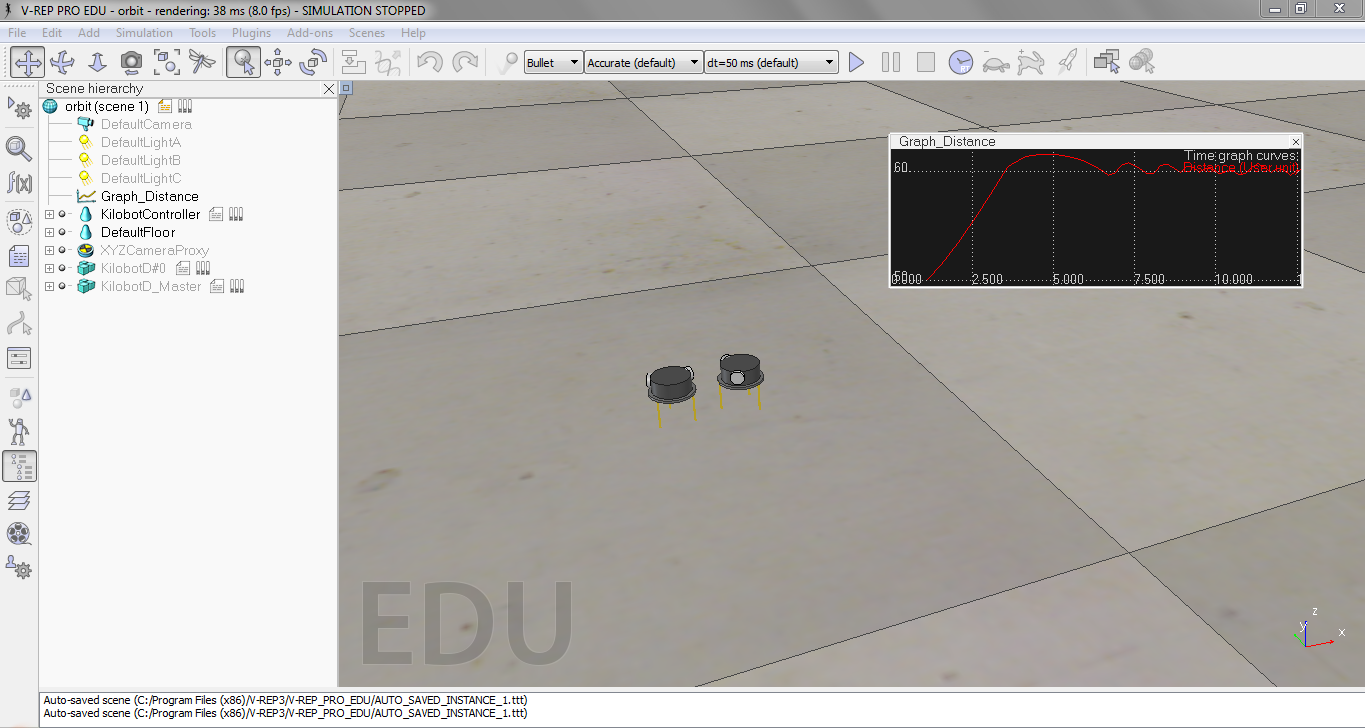
\includegraphics[width=16cm]{images/V-Rep.png}}
    \caption{Interface du simulateur V-Rep}
\end{figure}

\medskip
Malheureusement, le simulateur V-Rep ne r\'epond pas \`a nos besoins pour la simulation d'algorithme collectif sur les kilobots. Plusieurs probl\`emes furent rencontr\'es : \\ 

\medskip
Le langage utilis\'e pour les script est le Lua. Bien que tr\`es similaire au langage C, il nous oblige \`a retranscrire chaque programme en Lua. De plus, le fichier contenant le script en lua est incorpor\'e dans le fichier contenant la sc\`ene du simulateur (la sc\`ene comprend les mod\`eles de robot simul\'e, l'environnement ainsi que l'ensemble des scripts). C'est \`a la fois un avantage (partage d'une simulation tr\`es facile : tout est regroup\'e dans un seul fichier) et un inconv\'enient (obliger de partager l'ensemble de la sc\`ene pour pouvoir travailler en groupe et ne pas pouvoir travailler sur le script sans installer ou ex\'ecuter le simulateur).\\

\medskip
Le simulateur dispose lors de la simulation de plusieurs vitesses de simulation. Il est alors utile de pouvoir acc\'el\'erer le temps pour voir si l'impl\'ementation de l'algorithme est robuste et stable. Sauf que l'augmentation de la vitesse de simulation engendre des bugs dans le d\'eroulement des scripts et ne permet pas de s'assurer du bon fonctionnement d'un programme de mani\`ere fiable.\\

\medskip
Enfin, V-Rep est un simulateur orient\'e m\'ecanique. Il dispose en effet d'un moteur physique et d'un environnement en 3 dimensions pour pouvoir simuler des robots complexes comme des bras robotiques. Nous l'utilisons pour effectuer des simulations d'algorithmes, donc comme un simulateur logique. Il n'est alors pas adapt\'e \`a nos besoins (trop lourd, langage de script trop contraignant, nombreux bug durant la simulation).\\

\subsubsection*{KbSim}\label{subsubsec:name}
\addcontentsline{toc}{subsubsection}{KbSim}

\medskip
Nous avons alors cherché un autre simulateur et avons trouvé \textit{\textbf{KbSim}}\footnote{https://github.com/ajhalme/kbsim}, un simulateur entièrement dédié aux kilobots et développé en python en utilisant la librairie pygame.\\
Bien que n'utilisant pas les mêmes fichiers que les kilobots, sa programmation en python est aisée et permet une implémentation rapide des algorithmes dans le simulateur. Il offre aussi d'autre fonctionnalités comme par exemple l'affichage du rayon d'émission de chaque kilobot. Sa consommation plus faible en ressource et sa plus grande portabilité en font un simulateur plus adapté pour notre tâche que le simulateur V-Rep.\\

\begin{figure}[!h]
    \centering
    \subfigure{ 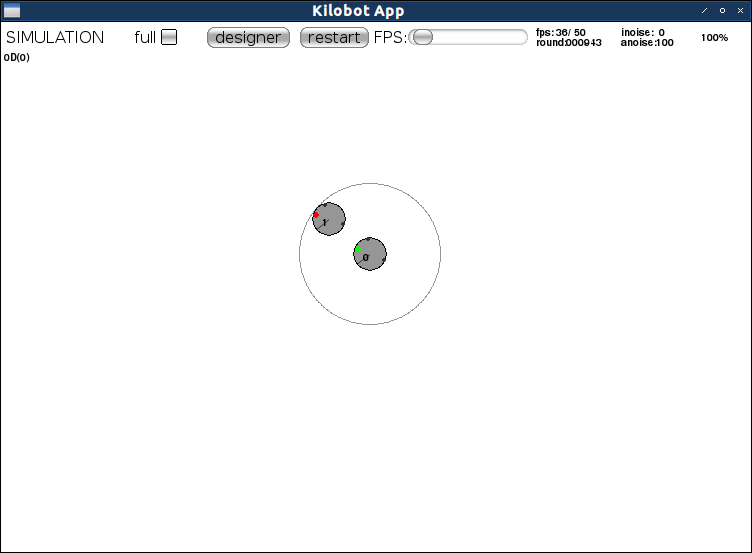
\includegraphics[width=14cm]{images/KbSim.png}}
    \caption{Interface du simulateur KbSim}
\end{figure}

\newpage
\subsection*{Firmware}\label{subsec:name}
\addcontentsline{toc}{subsection}{Firmware}

\subsubsection*{K-Team}\label{subsubsec:name}
\addcontentsline{toc}{subsubsection}{K-Team}

Les kilobots sont un mod\`ele de robots d\'evelopp\'es par l'universit\'e d'Harvard\footnote{http://www.eecs.harvard.edu/ssr/projects/progSA/kilobot.html}. L'entreprise suisse \textit{\textbf{K-Team}}\footnote{http://www.k-team.com/mobile-robotics-products/kilobot} les proposent \`a la vente et s'occupe de la fabrication et de l'assemblage. Ils fournissent les robots avec leur propre firmware d\'evelopp\'e en interne par la K-Team. \\
Ce firmware poss\`ede un inconv\'enient : il est compatible uniquement sous windows. \\
En effet, pour que l'op\'erateur puisse charger le programme dans les kilobots, il doit passer par le contr\^oleur qui est l'interface entre l'ordinateur et les robots. Or, le driver du contr\^oleur est uniquement disponible pour Windows et la K-Team ne fournit pas les sources pour un portage sous Linux. \\
De plus, nous avons rencontr\'e des probl\`emes lors de la calibration des moteurs avec le firmware d'origine. Ce dernier ne permet la calibration uniquement du moteur gauche ou du moteur droit mais pas des deux lorsqu'on souhaite avancer. Or, le positionnement des jambes de chaque kilobot n'\'etant pas parfaitement identique, nous avons besoin de valeurs diff\'erentes pour les deux moteurs afin que le robot se d\'eplace en ligne droite.\\

\subsubsection*{Kilobotics}\label{subsubsec:name}
\addcontentsline{toc}{subsubsection}{Kilobotics}

Apr\`es recherche, nous d\'ecid\^ames d'utiliser le firmware \textit{\textbf{Kilobotics}}\footnote{https://www.kilobotics.com/}. Kilobotics est le nom de la librairie d\'evelopp\'ee par l'universit\'e d'Harvard. Il est open-source et est plus r\'ecent et dispose d'un driver pour Linux. De plus, son utilisation limite les risques pour le mat\'eriel. Le contr\^oleur permet de charger les programmes dans les kilobots. Mais pour effectuer cela avec le firmware d'origine de la K-Team, il faut \`a chaque nouveau programme reprogrammer le microcontr\^oleur du contr\^oleur, ce qui implique le risque de se retrouver avec un microcontr\^oleur mal programm\'e et alors un contr\^oleur potentiellement hs. Le firmware kilobotics n\'ecessite lui de ne le reprogrammer qu'une seule fois, ce qui limite grandement les risques. \\
En ce qui concerne la calibration, kilobotic permet via l'interface graphique (\textbf{KiloGUI}) de calibrer chaque moteur s\'epar\'ement mais aussi de leur attribuer des valeurs diff\'erentes pour le d\'eplacement en ligne droite. Kilogui propose aussi la possibilit\'e de rentrer directement les valeurs souhait\'ees (entre 1 et 255) pour la puissance des moteurs. Enfin, il est possible d'affecter un identifiant \`a chaque robot qui sera stock\'e dans la m\'emoire EPROM.\\

\begin{figure}[!h]
    \centering
    \subfigure{ 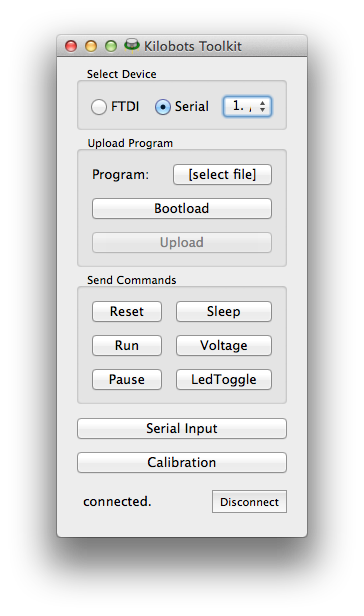
\includegraphics[width=10cm]{images/KiloGUI.png}}
    \subfigure{ 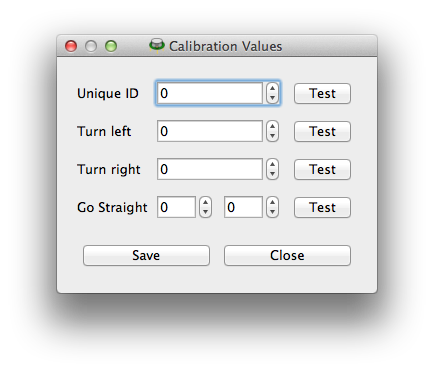
\includegraphics[width=10cm]{images/calib.png}}
    \caption{Interface de l'application KiloGUI}
\end{figure}

%%%%%%%%%%%%%%%%%%%%%%%%%%%%%%%%%%%%%%%%%%%%%%%%%%%%%%%%%%%%%%%%%%
%                                                                %
%                           PHASE I                              %
%                                                                %
%%%%%%%%%%%%%%%%%%%%%%%%%%%%%%%%%%%%%%%%%%%%%%%%%%%%%%%%%%%%%%%%%%
\chapter{Phase I}

Ce projet se d\'ecoupe en 3 phases :

\begin{enumerate}[{Phase}-1 ]
\item \textit{\textbf{Recherche Documentaire et Prise en main}}.
\item \textit{\textbf{Recherche d'un bio-algorithme et d\'eveloppement}}.
\item \textit{\textbf{Impl\'ementation d'un mod\`ele de robot avec les kilobots}}.
\end{enumerate}

\bigskip
La phase I ne comprenant que de la recherche documentaire et la prise en main de la plate-forme, la r\'epartition se deroula ainsi, Arnaud prit en main la plate-forme et Benjamin la recherche documentaire.\\
Pour la prise en main de la plate-forme, deux algorithmes fut choisis mettant chacun en scène une ou plusieurs capacit\'es: la locomotion et la communication.\\
Le premier algorithme est celui de l'orbite. Il permet de d\'eplacer de façon circulaire un kilobot autour d'un point repr\'esenter par un autre robot.\\
Le second met en avant la communication entre eux et se nomme firefly. Il r\'ealise une synchronisation de plusieurs horloges (ici celles de plusieurs robots) via \'echange de messages.\\

\section*{Orbite}\label{sec:name}
\addcontentsline{toc}{section}{Orbite}

L'orbite reprend le principe des satellites naturels comme la lune qui tourne autour de la terre. Chaque astre prend ici la forme d'un kilobot. Le premier va effectuer une r\'evolution autour du second pendant que ce dernier lui enverra des messages en continu. L'emploi d'un second kilobot est indispensable pour permettre à un autre d'avancer en formant un cercle. Sans point de repère, il est impossible d'en effectuer un correctement, les d\'eplacements par vibrations \'etant trop impr\'ecis et entraînant des mouvements non d\'esir\'es. La surface sur laquelle \'evolue le robot rajoute encore un facteur impr\'evisible.

Un kilobot va rester en position stationnaire et envoyer des messages en continue. Le contenu de ceux-ci n'est d'aucune importance. Ils ne servent qu'\`a transmettre la distance qui s\'epare l’\'emetteur des r\'ecepteurs.\\
Le second kilobot va lui avancer en continu et recevoir les messages du premier. A chaque r\'eception, il va calculer la distance qui le s\'epare de l'\'emetteur et ainsi pouvoir faire des corrections de trajectoire. Il avance ainsi tout droit tant qu'il se trouve dans les bornes d\'efinies dans le programme. S'il se trouve à une distance inf\'erieure à celle-ci, il tournera à gauche jusqu’à de nouveau être dans les bornes. Il effectuera la même op\'eration s'il est à une distance sup\'erieure, mais vers la droite.\\
Ainsi, il va naturellement r\'ealiser une r\'evolution autour du kilobot fixe en tournant autour.\\

\newpage
\begin{center}
  \rule{\linewidth}{.5pt}
  \textbf{Orbite}\\
  \rule{\linewidth}{.5pt}
\end{center}
\underline{Legende} : \textbf{S} (Send) et \textbf{R} (Receive).\\

\begin{table}[h]
\begin{tabular}{lllll}
\textit{Master} &                          &  & \textit{Slave} &                                                                                                                                                                                                                                                          \\
                &                          &  &                &                                                                                                                                                                                                                                                          \\
\textbf{S :}    & envoie un message $<$$>$ &  & \textbf{S :}   &                                                                                                                                                                                                                                                          \\
\textbf{R :}    &                          &  & \textbf{R :}   & r\'eception d'un message $<>$                                                                                                                                                                                                               \\
                &                          &  &                & \begin{tabular}[c]{@{}l@{}} Si distance \textgreater= distance\_max\\ tourner à droite\\ avancer tout droit\\ Sinon SI distance \textless= distance\_min\\      touner à gauche \\ avancer tout droit\\ Sinon\\ avancer tout droit\\ Fin Si \end{tabular}
\end{tabular}
\end{table}

Le kilobot \textit{Master} reste immobile tandis que le kilobot \textit{Slave} orbite autour de lui.\\

\section*{Firefly}\label{sec:name}
\addcontentsline{toc}{section}{Firefly}

L'algorithme firefly est un bio-algorithme s'inspirant du comportement des lucioles dans la nature. Quand elles se retrouvent en groupe, elles sont capables de "clignoter" de manière synchronis\'ee.
Les kilobots font de même avec cet algorithme.\\

Pour permettre possible la synchronisation de plusieurs individus, nous impl\'ementons une horloge logique dans chacun. La synchronisation va se r\'ealiser en collectant les horloges contenues dans les messages des voisins afin de d\'eterminer la moyenne du nombre de tick d'horloge qui sont en avance (ou en retard).\\

Le kilobot dispose donc d'un tableau dont les indexes sont le nombre de tick en retard ou en avance par rapport à ses voisins.\\
Exemple : Si la diff\'erence entre son horloge et l'horloge reçue dans un message est de 8 ticks, alors il incr\'ementera de 1 la valeur contenue à l'index 8 du tableau.\\
Le tableau est ainsi mis à jour à chaque r\'eception d'un message seulement si la diff\'erence entre l'horloge de l’\'emetteur et celle du r\'ecepteur est inf\'erieure à la moiti\'e de la p\'eriode d'horloge. Cette pr\'evention permet d'\'eviter que deux kilobots voisins se mettent à jour en même temps.\\

A chaque it\'eration de la boucle principale du programme, la moyenne de la somme des ticks enregistr\'es dans le tableau est effectu\'ee (tick\_offset) et celui-ci remis à z\'ero. La diff\'erence entre l'horloge locale (kilo\_ticks) et celle reçue est calcul\'ee :\\

modulo\_clock = ((kilo\_ticks – tick\_offset) / 4) \% 32\\

Si modulo\_clock est \'egale à z\'ero, le robot peut alors faire clignoter sa led. 
Ainsi la synchronisation se fait au fil des cycles en r\'eduisant l'\'ecart entre chaque horloge.

\newpage
\begin{center}
  \rule{\linewidth}{.5pt}
  \textbf{Luciole/Firefly}\\
  \rule{\linewidth}{.5pt}
\end{center}
\underline{Legende} : \textbf{S} (Send) et \textbf{R} (Receive).\\

\begin{table}[h]
\begin{tabular}{lllll}
\textbf{S :} & envoie un message $<$Horloge$>$ &  & \textbf{R :} & r\'eception d'un message $<$Horloge$>$                                                                                                                                                                             \\
           &                                   &  &            & \begin{tabular}[c]{@{}l@{}}Si mon\_Horloge \textgreater Horloge            \\     d\'ecr\'ementation de mon\_Horloge d'une demi-p\'eriode\\ Sinon    \\     incr\'ementation de mon\_Horloge d'une demi-p\'eriode\\ Fin Si\end{tabular} \\
\end{tabular}
\end{table}

%%%%%%%%%%%%%%%%%%%%%%%%%%%%%%%%%%%%%%%%%%%%%%%%%%%%%%%%%%%%%%%%%%
%                                                                %
%                           PHASE II                             %
%                                                                %
%%%%%%%%%%%%%%%%%%%%%%%%%%%%%%%%%%%%%%%%%%%%%%%%%%%%%%%%%%%%%%%%%%
\chapter{Phase II}


La phase II demandant plus de r\'eflexion, nous m\^imes nos comp\'etences acquises \`a la premi\`ere phase en commun afin de proposer un bio-algorithme digne d'int\'er\^et.

\section*{Phototaxis}\label{sec:name}
\addcontentsline{toc}{section}{Phototaxis}

Notre bio-algorithme se base sur le principe de phototaxis.\\

\smallskip
\textit{R\'eaction de locomotion d'organismes mobiles provoqu\'ee par la lumi\`ere et qui les porte soit \`a s'en approcher (phototaxie positive), soit \`a s'en \'eloigner (phototaxie n\'egative).}\\

\smallskip
Notre algorithme ne permet pas une entraide des kilobots, c'est \`a dire que chaque robot suit son programme sans se soucier des autres.\\
Cette version ne permet donc pas \`a un essaim en formation de suivre la lumi\`ere tout en gardant cette formation.\\
L'algorithme se d\'eroule ainsi, chaque robot capte la lumi\`ere ambiante (la lumi\`ere ambiante doit \^etre faible afin de ne pas g\^ener les capteurs des kilobots dans la d\'etection de la source cible de lumi\`ere), si la source de lumi\`ere d\'etect\'ee par le capteur provient de la droite on tourne \`a droite et inversement, apr\`es chaque demi-tour on avance tout droit pendant un certain laps de temps.\\
Les kilobots ne communiquent jamais ensemble.\\

\newpage
\begin{center}
  \rule{\linewidth}{.5pt}
  \textbf{Phototaxis}\\
  \rule{\linewidth}{.5pt}
\end{center}

\begin{verbatim}
var currentLight <- indice de lumière ambiante.
var currentDir   <- indice de direction.

Tant que vrai   
     r\'eception de la lumière

     Si currentLight > barrière haute
     alors
        -tourner à droite
        -currentDir <- droite;
     Fin Si
 
     Si currentLight < barrière basse
     alors
        -tourner à gauche
        -currentDir <- gauche;
     Fin Si
Fin Tant que
\end{verbatim}

%La seconce version de notre algorithme utilise l'algorithme de gradient afin de garder les kilobots en formation jusqu'\`a la source de lumi\`ere.\\
%Par exemple les kilobots ont une formation en A, et ils doivent garder cette forme jusqu'\`a la destination.\\

\section*{Gradient}\label{sec:name}
\addcontentsline{toc}{section}{Gradient}

L'algorithme du gradient permet de calculer sa distance par rapport à une balise fixe.\\
Chaque kilobot transmet à tous ses voisins la distance qui le s\'epare de la balise. Ainsi, chaque robot peut calculer sa propre distance par rapport à la balise sans pour autant communiquer directement avec elle. L'ensemble des robots sert de relais pour la balise fixe.\\
Une fois sa distance calcul\'ee, le kilobot allume sa led pour signaler sa position.

\medskip
\begin{figure}[!h]
    \centering
    \subfigure{ 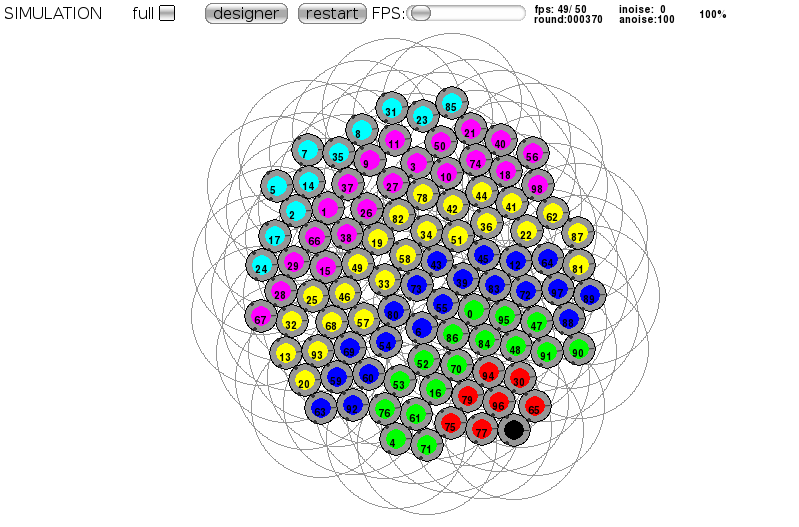
\includegraphics[width=14cm]{images/gradient.png}}
    \caption{Gradient à une balise}
\end{figure}

\newpage
\begin{center}
  \rule{\linewidth}{.5pt}
  \textbf{Gradient}\\
  \rule{\linewidth}{.5pt}
\end{center}

\begin{verbatim}
var timer
var gradient_value

Tant que vrai
     attendre une seconde
     incr\'ementer timer
     Si timer >= 5000 // Actualisation toutes les 5 secondes
     alors
          Si kilo_uid == 0 // Si le kilobot a l'id 0.
          alors
               gradient_value <- 0
          Sinon
               gradient_value <- Valeur maximum
          Fin si
          timer <- 0
     Fin si

     Si nouveau message
     alors
          Si gradient_value > valeur_reçue + 1
          alors
               gradient_value <- valeur_reçue + 1
               mettre à jour le message à envoyer.
               timer <- 0
          Fin si

          Switch(gradient_value % 3)
               0 -> allumer led en rouge
               1 -> allumer led en vert
               2 -> allumer led en bleu
          Fin switch
     Fin si
Fin tant que
\end{verbatim}

%%%%%%%%%%%%%%%%%%%%%%%%%%%%%%%%%%%%%%%%%%%%%%%%%%%%%%%%%%%%%%%%%%
%                                                                %
%                           PHASE III                            %
%                                                                %
%%%%%%%%%%%%%%%%%%%%%%%%%%%%%%%%%%%%%%%%%%%%%%%%%%%%%%%%%%%%%%%%%%
\chapter{Phase III}

\section*{Modèle CORDA}\label{sec:name}
\addcontentsline{toc}{section}{Modèle CORDA}

Cette phase vise \'a rechercher le moyen d'impl\'ementer le \textbf{mod\`ele CORDA}\footnote{Giuseppe Prencipe. A new distributed model to control and coordinate a set of autonomous mobile robots : The corda model, 2000.}.\\

\smallskip
Comme définis dans l'article \textit{Nettoyage perpétuel de réseaux}, le modèle CORDA est un modèle asynchrone. Chaque entité est autonome et agit par cycles asynchrones.\\

%DEBUT CITE

\textit{"Un cycle est constitu\'e de 3 phases : Voir, Calculer et Agir. Chaque phase est ex\'ecut\'ee de mani\`ere atomique et asynchrone. Une entit\'e a d’abord acc\`es \`a vue, du r\'eseau, comprenant la topologie du r\'eseau et les positions des autres entit\'es dans le r\'eseau \`a un moment donn\'e (Phase Voir). Sur la base de ces informations, l’entit\'e peut effectuer un calcul (Phase Calculer) et en d\'eduire une action : se d\'eplacer ou non sur un sommet voisin (Phase Agir)."}\footnote{L\'elia Blin, Janna Burman, and Nicolas Nisse. Nettoyage perpétuel de réseaux. In Nicolas Matheieu, Fabien et Hanusse, editor, 14`mes Rencontres Francophones sur les Aspects Algorithmiques des Télécommunications (AlgoTel), page 4, La Grande Motte, France, 2012.}\\

%FIN CITE

Nous avons choisi de nous pencher sur ce mod\`ele pr\'ecis car ce mod\`ele est largement utilis\'e pour les algorithmes r\'eparties dans le domaine de la robotique.\\

Il d\'efinit des caract\'eristiques physiques dont devront disposer les robots :

\begin{itemize}
\item chaque robot poss\`ede un rep\`ere orthonorm\'e.
\item chaque robot poss\`ede une vision "infinie".
\item chaque robot ne poss\`ede aucun moyen de communiquer avec ses cong\'en\`eres.
\item chaque d\'eplacement du robot est pr\'ecis.
\end{itemize}

\medskip
Ces contraintes posent plusieurs probl\`ematiques. En effet la plate-forme Kilobot ne propose aucune de ces caract\'eristiques. (cf chapitre 2)\\
Donc comment simuler une vision "infinie" avec la plate-forme Kilobot ? Comment simuler un axe orthonorm\'e ? Comment localiser les robots les uns par rapport aux autres ? Et plus important comment un robot peut se localiser dans l'espace ?\\

\section*{Impl\'ementation}\label{sec:name}
\addcontentsline{toc}{section}{Impl\'ementation}

Nous pouvons r\'esoudre le probl\`eme de la localisation dans l'espace (ainsi que la localisation par rapport aux autres) et de l'axe orthonorm\'e en utilisant la m\'ethode de la trilat\'eration. Les robots Kilobot ne poss\`edent pas de cam\'era et ont une port\'ee de communication limit\'ee ce qui nous ne permet pas d'impl\'ementer un vision infinie \`a proprement parler.\\

\subsection*{Premi\`ere Approche}\label{sec:name}
\addcontentsline{toc}{subsection}{Premi\`ere Approche}

Nous pouvons, de mani\`ere na\"{i}ve, r\'esoudre le probl\`eme de localisation des robots en disposant des balises sur un cercle de diam\`etre 14cm (cf figure : ~\ref{figureI}), en effet la distance maximum d'\'emmission de messages est de 7cm donc le diam\`etre maximal du cercle est donc bien de 14cm.\\
Chaque point de la figure repr\'esente une balise, et les cercles permettent de visualiser les zones de communications.\\
Nous remarquons que l'ajout de cinq balises sur le cercle ne nous permet pas de recouvrir de mani\`ere optimale la zone (int\'erieur du cercle) donc nous doublons le nombre de balises.\\
Cela permet effectivement de couvrir toute la zone et de localiser de mani\`ere "pr\'ecise".\\
Notre approche r\'esout le probl\`eme de la localisation mais pose un autre probl\`eme. Comment augmenter la zone de travail?\\
En effet, la zone couverte permet de faire fonctionner correctement seulement deux kilobots.\\
Donc notre approche n'est pas viable pour simuler le mod\`ele CORDA sur la plate-forme Kilobot.\\

\begin{figure}[!h]
    \centering
    \subfigure{ 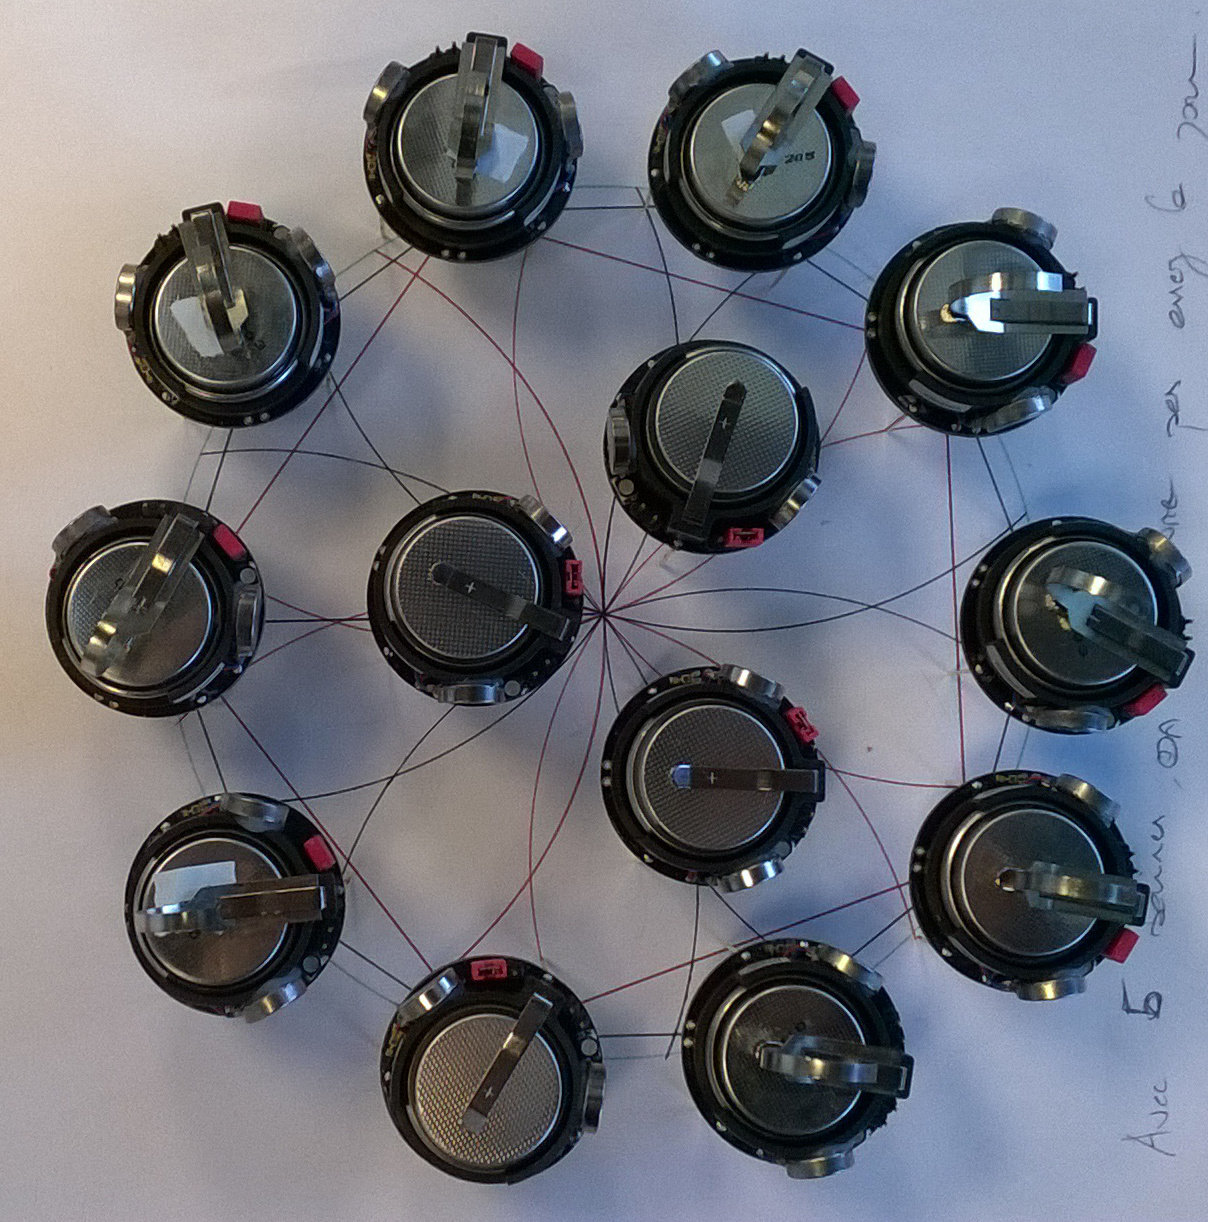
\includegraphics[width=14cm]{images/locate_bounding_box_demo.jpg}}
    \caption{Simulation de la première approche}
\end{figure}

%%%%%%%
% IMAGES des robots avec la premiere approche
%%%%%%%

\begin{figure}
  \begin{tikzpicture}
    %%%%%%%%%%%%%%%%%%%%%%%%%%%%%%%%%%%%%%%
    %           VARIABLE RAYON            %
    %%%%%%%%%%%%%%%%%%%%%%%%%%%%%%%%%%%%%%%
    \newcommand{\rayon}{4}

    %%%%%%%%%%%%%%%%%%%%%%%%%%%%%%%%%%%%%%%
    %        AVEC 5 BALISES               %
    %%%%%%%%%%%%%%%%%%%%%%%%%%%%%%%%%%%%%%%
    %\draw[line width=3pt] (0,0) -- (0,\rayon);                % 0 -> A
    \draw[red,line width=2pt] (0,\rayon) -- (18:\rayon);      % A -> B
    \draw[red,line width=2pt] (18:\rayon) -- (-54:\rayon);    % B -> C
    \draw[red,line width=2pt] (-54:\rayon) -- (-126:\rayon);  % C -> D
    \draw[red,line width=2pt] (-126:\rayon) -- (-198:\rayon); % D -> E
    \draw[red,line width=2pt] (-198:\rayon) -- (0,\rayon);    % E -> A
    
    %%%%%%%%%%%%%%%%%%%%%%%%%%%%%%%%%%%%%%%
    %        AVEC 10 BALISES              %
    %%%%%%%%%%%%%%%%%%%%%%%%%%%%%%%%%%%%%%%
    \draw[blue,line width=2pt] (0,\rayon) -- (54:\rayon);       % A  -> AB
    \draw[blue,line width=2pt] (54:\rayon) -- (18:\rayon);      % AB -> B
    \draw[blue,line width=2pt] (18:\rayon) -- (-18:\rayon);     % B  -> BC
    \draw[blue,line width=2pt] (-18:\rayon) -- (-54:\rayon);    % BC -> C
    \draw[blue,line width=2pt] (-54:\rayon) -- (-90:\rayon);    % C  -> CD
    \draw[blue,line width=2pt] (-90:\rayon) -- (-126:\rayon);   % CD -> D
    \draw[blue,line width=2pt] (-126:\rayon) -- (-162:\rayon);  % D  -> DE
    \draw[blue,line width=2pt] (-162:\rayon) -- (-198:\rayon);  % DE -> E
    \draw[blue,line width=2pt] (-198:\rayon) -- (-234:\rayon);  % E  -> EA
    \draw[blue,line width=2pt] (-234:\rayon) -- (0,\rayon);     % EA -> A

    %%%%%%%%%%%%%%%%%%%%%%%%%%%%%%%%%%%%%%%
    %         ARC avec 5 balises          %
    %%%%%%%%%%%%%%%%%%%%%%%%%%%%%%%%%%%%%%%
    \draw[densely dashdotdotted,red] (0,\rayon) circle (\rayon);
    \draw[densely dashdotdotted,red] (18:\rayon) circle (\rayon);
    \draw[densely dashdotdotted,red] (-54:\rayon) circle (\rayon);
    \draw[densely dashdotdotted,red] (-126:\rayon) circle (\rayon);
    \draw[densely dashdotdotted,red] (-198:\rayon) circle (\rayon);

    %%%%%%%%%%%%%%%%%%%%%%%%%%%%%%%%%%%%%%%
    %         ARC avec 10 balises         %
    %%%%%%%%%%%%%%%%%%%%%%%%%%%%%%%%%%%%%%%
    \draw[densely dashdotdotted,blue] (54:\rayon) circle (\rayon);
    \draw[densely dashdotdotted,blue] (-18:\rayon) circle (\rayon);
    \draw[densely dashdotdotted,blue] (-90:\rayon) circle (\rayon);
    \draw[densely dashdotdotted,blue] (-162:\rayon) circle (\rayon);
    \draw[densely dashdotdotted,blue] (-234:\rayon) circle (\rayon);

    %%%%%%%%%%%%%%%%%%%%%%%%%%%%%%%%%%%%%%%
    %               INIT                  %
    %%%%%%%%%%%%%%%%%%%%%%%%%%%%%%%%%%%%%%%
    \draw[line width=3pt] (0,0) circle (\rayon);
    
    \draw (0,\rayon) node[above]{$A$};
    \draw (18:\rayon.2) node[above]{$B$};
    \draw (-54:\rayon.2) node[right]{$C$};
    \draw (-126:\rayon.2) node[below]{$D$};
    \draw (-198:\rayon.2) node[left]{$E$};
    
    \draw (54:\rayon.2) node[above]{$AB$};
    \draw (-18:\rayon.2) node[right]{$BC$};
    \draw (-90:\rayon.2) node[below]{$CD$};
    \draw (-162:\rayon.2) node[left]{$DE$};
    \draw (-234:\rayon.2) node[left]{$EA$};
    
  \end{tikzpicture}
  \caption{Premi\`ere Approche}
  \label{figureI}
\end{figure}

\newpage
\subsection*{Seconde Approche}\label{sec:name}
\addcontentsline{toc}{subsection}{Seconde Approche}

La premi\`ere approche r\'esolvait le probl\`eme de localisation et de positionnement, mais ne permettait pas de faire fonctionner plus de deux robots de mani\`ere viable.\\
Donc notre deuxi\`eme approche devra, elle aussi, r\'esoudre le probl\`eme de localisation et de positionnement mais devra, par contre, agrandir la zone de travail des robots (par exemple de permettre \`a 6 robots ou plus d'\^etre dans la zone de travail sans se g\^ener).\\

\medskip
Nous pouvons utiliser la m\'ethode dite de \textbf{"bounding box"}\footnote{Thomas Moinel. Coordination d’un essaim de robots mobiles (30 kilobots) par des m\'́ecanismes inspir\'́es de l’intelligence collective observ\'́ee chez les animaux sociaux. 2012}.\\
La m\'ethode par "bounding box" consiste \`a calculer la position, ici d'un robot, par l'intersection des zones des balises.

\begin{figure}[!h]
    \centering
    \subfigure{ 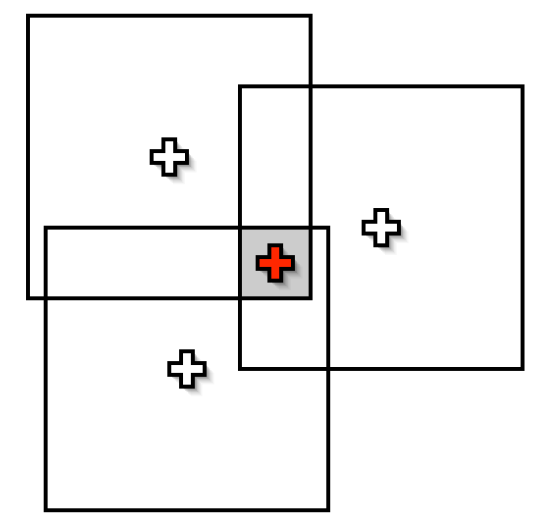
\includegraphics[width=8cm]{images/bounding.png}}
    \caption{Exemple de "bounding box"}
\end{figure}

Cette m\'ethode augmenterait le nombre de balises par rapport au nombre de robots utiles de mani\`ere trop importante (du faite de la faible distance de communication des Kilobots).\\
Nous pouvons utiliser la \textbf{m\'ethode de multilat\'eration}.\\
La multilat\'eration est une technique de positionnement ayant recours \`a des balises fixes dont les positions sont connues. Elle se base sur les diff\'erences de distance entre deux balises lorsqu'elles emettent des messages \`a intervalles r\'eguliers\footnote{http://en.wikipedia.org/wiki/Multilateration}.\\
Cette m\'ethode ne demande que trois balises et aucune connectivit\'e directe avec les balises (la distance est estim\'ee gr\^ace \`a la propagation d'un gradient) mais cette m\'ethode pose le probl\`eme de la puissance de calcul, en effet la plate-forme Kilobot offre une puissance de calcul limit\'ee ne permettant pas d'impl\'ementer cette m\'ethode.\\

\smallskip
La solution serait de proposer une m\'ethode hybride entre ces deux m\'ethodes, soit la m\'ethode de "bounding box" avec la distance estim\'ee avec un gradient.\\
Cette solution permettra \`a terme d'agrandir la zone de travail mais aura comme cons\'equence une perte de pr\'ecision.\\


\section*{Sp\'ecifications de l'API}\label{sec:name}
\addcontentsline{toc}{section}{Fonctions de l'API}

Nous proposons l'impl\'ementation d'une API permettant de simuler le mod\`ele CORDA, elle devra comprendre les primitives suivantes :

\begin{description}
\item[getPosition] qui permet \`a un robot de conna\^itre sa position.
\item[getVision] qui permet \`a un robot de conna\^itre la position des robots qui l'entourent.
\item[toPosition] qui permet \`a un robot de se rendre aux coordonn\'ees en param\`etre.
\end{description}

\smallskip
Cette API s'appuiera sur l'API existante de Kilobotics.\\

\subsection*{getPosition}\label{sec:name}
\addcontentsline{toc}{subsection}{getPosition}

Cette primitive se basera sur l'algorithme du gradient vu précédemment. Elle permetra de connaître la position du robot par rapport aux balises. En effet, le gradient forme une grille qui est utilisée par les robots pour calculer leur position. En le couplant au "bounding box", nous pouvons obtenir une méthode de localisation demandant moins de balises et augmentant aussi la surface couverte par la grille. De plus, cette technique est compatible avec les limitations matérielles des kilobots au niveau "hardware" (puissance de calcul).

\subsection*{getVision}\label{sec:name}
\addcontentsline{toc}{subsection}{getVision}

Cette primitive récupère la position de l'ensemble des kilobots voisins pour un kilobot donné. En connaissant les positions des voisins, il sera possible de simuler un cône de vision pour respecter la contrainte du modèle CORDA.

\subsection*{toPosition}\label{sec:name}
\addcontentsline{toc}{subsection}{toPosition}

Cette dernière primitive réunie les deux précédentes afin de proposer un système de déplacement vers une position donnée pour un ensemble de robots.\\

\bigskip
\section*{Avancement du projet}\label{sec:name}
\addcontentsline{toc}{section}{Avancement du projet}

Durant ces 4 mois durant lesquels nous avons travaillé sur le projet, nous avons pu réaliser les deux premières phases demandées. Au vue de notre avancement dans le projet, ils nous fût proposés de commencer une troisième phases orientée recherche et qui est toujours en cours. En effet, nous avons réalisé un travail de recherche sur les différentes possiblités pour implémenter le modèle CORDA. Au jour de la rédaction de ce rapport, seule la primitive getPosition est en cours d'implémentation. Elle devrait être disponible ultérieurement sur le github du projet\footnote{https://github.com/LSDev8/PSAR-Kilobot}.\\

\smallskip
La dernière phase de ce projet a aussi été l'occasion pour nous d'avoir un bref aperçu du monde de la recherche.
Nous fûment confrontés aux al\'eas du chercheur, \`a savoir une grande recherche bibliographique et \`a la contrari\'et\'e de voir de nombreuses pistes devenir infructeuses.\\

%                            __
%                          .'`  `.      __
%                         /      |  ,-'`  `'.
%                        ;       '-'         )
%                        |              _,.-'
%                    _   |_.--.,       (_
%                 .'` `'-'__    \        ''"'-.
%                /  .-"-/`  `\   ;_            \
%                | /   ;      ;  | `.   (`'.__.'
%                 |   o| o    | __   \   `.
%           _,.---'\___.\.__.'    `'. |_   )
%       _.-'               _.-""-.   '-.'-'
%     ,'                     |   \`.    `.
%    /                       ;   |       |
%   (_.-'""''---..           /   |      /
%                 `'-..___.-'    ;  ,.-'
%                       \ 7      ' / |
%                       |/_  _  ; /  '
%                   .-  /' /` j/ '   |
%                   | \|  '   /  |
%                   '  `.___.'  ;     '
%                   ;          /      |
%                    \        /       |
%                     `.,__,.'         '
%                        |             |
%                        ;              '
%                       /                |
%                      ' ___________ ...-'

%%%%%%%%%%%%%%%%%%%%%%%%%%%%%%%%%%%%%%%%%%%%%%%%%%%%%%%%%%%%%%%%%%
%                                                                %
%                          ANNEXE                                %
%                                                                %
%%%%%%%%%%%%%%%%%%%%%%%%%%%%%%%%%%%%%%%%%%%%%%%%%%%%%%%%%%%%%%%%%%
\chapter{Annexe}

\section*{Mat\'eriel Utilis\'e}\label{sec:name}
\addcontentsline{toc}{section}{Mat\'eriel Utilis\'e}

Le mat\'eriel se compose des kilobots, de transmetteur et d'un PC quelqu'il soit.

\section*{Logiciel Utilis\'e}\label{sec:name}
\addcontentsline{toc}{section}{Logiciel Utilis\'e}

Nous utiliserons les logiciels fournis pour l'API Kilobotics pour le d\'eveloppement de notre API, notre gestionnaire de version sera Github.\\
Le projet sera h\'eberg\'e sous l'organisation \textit{\textbf{LSDev8}}\footnote{https://github.com/LSDev8/}.\\
Nous utilisions (au d\'ebut du projet) pour nos simulations le logiciel \textit{\textbf{V-Rep}}\footnote{http://www.coppeliarobotics.com} mais celui-ci se r\'ev\'ela trop contraignant dans son utilisation donc nous opt\^ames pour le logiciel \textit{\textbf{KbSim}}\footnote{https://github.com/ajhalme/kbsim} car celui-ci est un simulateur exclusivement pour kilobot (une copie de ce logiciel se trouve aussi sur l'organisation \textit{\textbf{LSDev8}}).\\


\section*{Tutoriels}\label{sec:name}
\addcontentsline{toc}{section}{Tutoriels}

Au cours de notre projet, nous avons été confrontés à divers problèmes. Nous avons décidé de réunir les probl\`emes les plus r\'ecurrent sous forme de tutoriels afin d'en faire profiter ultérieurement toutes personnes qui s'y retrouverait confrontés.

\subsection*{Installation du contr\^oleur}\label{sec:name}
\addcontentsline{toc}{subsection}{Installation du contr\^oleur}

Le contr\^oleur exploite un microcontr\^oleur Atmega m328p. Lors de la première connexion du contr\^oleur \`a un ordinateur Windows, Windows va automatiquement aller t\'el\'echarg\'e les drivers correspondant via windows update et les installer. Il n'y a pas d'autre op\'erations \`a faire. Sous Linux, aucun driver n'est n\'ecessaire.\\
Si vous utilisez le firmware original de la K-Team, il vous faudra alors installer pour Windows un driver suppl\'ementaire afin de faire communiquer l'interface graphique avec le contr\^oleur. Pour cela, suivez les instructions fournies dans le manuel de la K-Team.

\begin{center}
  \fcolorbox{red}{white}{
    \begin{minipage}{1.0\textwidth}
      Si le contr\^oleur n'est pas reconnu par windows, assurez-vous qu'il appara\^it bien dans le gestionnaire de p\'eriph\'erique.\\ Il doit normalement appara\^itre comme un Serial Port (FTDI) et un AVRisp mkII (Jungo).
    \end{minipage}
  }
\end{center}

\subsection*{Flashage du contr\^oleur et des kilobots}\label{sec:name}
\addcontentsline{toc}{subsection}{Flashage du contr\^oleur et des kilobots}

Si vous d\'esirez passer au firmware kilobotics, il est n\'ecessaire d'utiliser le logiciel AvrDude. Ce logiciel d\'evelopp\'e par Atmel permet de reprogrammer le microcontr\^oleur du contr\^oleur. Pour cela, connecter le contr\^oleur \`a un ordinateur via un cable usb, ouvrer un terminal et placez-vous dans le r\'epertoire contenant le nouveau firmware (au format .hex) puis assurez-vous que le cavalier du contr\^oleur est bien positionn\'e en mode interne (c'est la position par d\'efaut : c'est \`a dire sur la gauche). \\

\begin{figure}[!h]
    \centering
    \subfigure{ 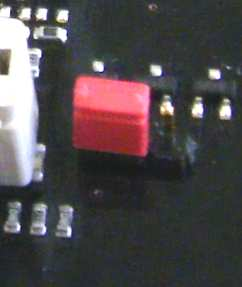
\includegraphics[width=8cm]{images/flashI.png}}
    \caption{Cavalier en position interne}
\end{figure}

Enfin, ex\'ecuter la commande suivante :\\

\begin{center}
  \textbf{avrdude -p m328  -P usb -c avrispmkII -U "flash:w:controller.hex:i"}
\end{center}

Pour flasher les kilobots, l'op\'eration est tr\`es similaire. Connecter le contr\^oleur, ouvrer un terminal et placez-vous dans le r\'epertoire contenant le nouveau firmware (toujours au format .hex). Placez cette fois-ci le cavalier du contr\^oleur en mode externe (sur la droite): \\

\begin{figure}[!h]
    \centering
    \subfigure{ 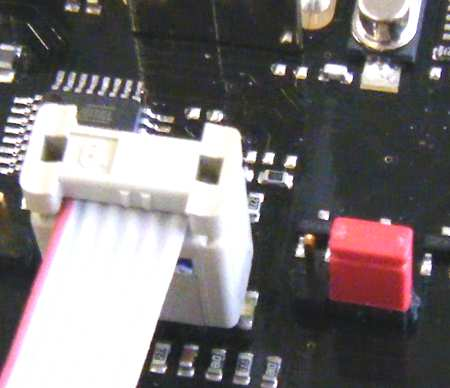
\includegraphics[width=8cm]{images/flashII.png}}
    \caption{Cavalier en position externe}
\end{figure}

Puis connecter le c\^able au contr\^oleur et au kilobot via les 6 trous pr\'esents sur le c\^ot\'e du kilobot.\\
Enfin, ex\'ecuter la commande suivante :\\

\begin{center}
  \textbf{avrdude -p m328p -P usb -c avrispmkII -U "flash:w:bootloader.hex:i"}
\end{center}

\smallskip
\begin{center}
  \fcolorbox{red}{white}{
    \begin{minipage}{1.0\textwidth}
      Si AvrDude ne reconnaît pas le contr\^oleur, assurez-vous d'avoir positionn\'e le cavalier dans la bonne position. Sinon, la connexion entre le connecteur du câble et le kilobot est tr\`es sensible. Il faut que toutes les broches du connecteur soit en contact avec le kilobot. N'h\'esitez surtout pas \`a presser l\'eg\`erement le connecteur contre le kilobot et \`a le placer l\'eg\`erement en biais afin d'assurer la bonne connexion entre le connecteur et le robot.
    \end{minipage}
  }
\end{center}

\newpage
\subsection*{Chargement des kilobots}\label{sec:name}
\addcontentsline{toc}{subsection}{Chargement des kilobots}

Les kilobots peuvent être recharg\'es via le chargeur de la K-Team. Pour cela, passez les en mode charge grâce au contrôleur et à l'interface graphique kilogui, puis disposez les sur le chargeur. Ils clignoteront en rouge pendant la charge puis passeront au bleu une fois la charge termin\'ee.

\begin{figure}[!h]
    \centering
    \subfigure{ 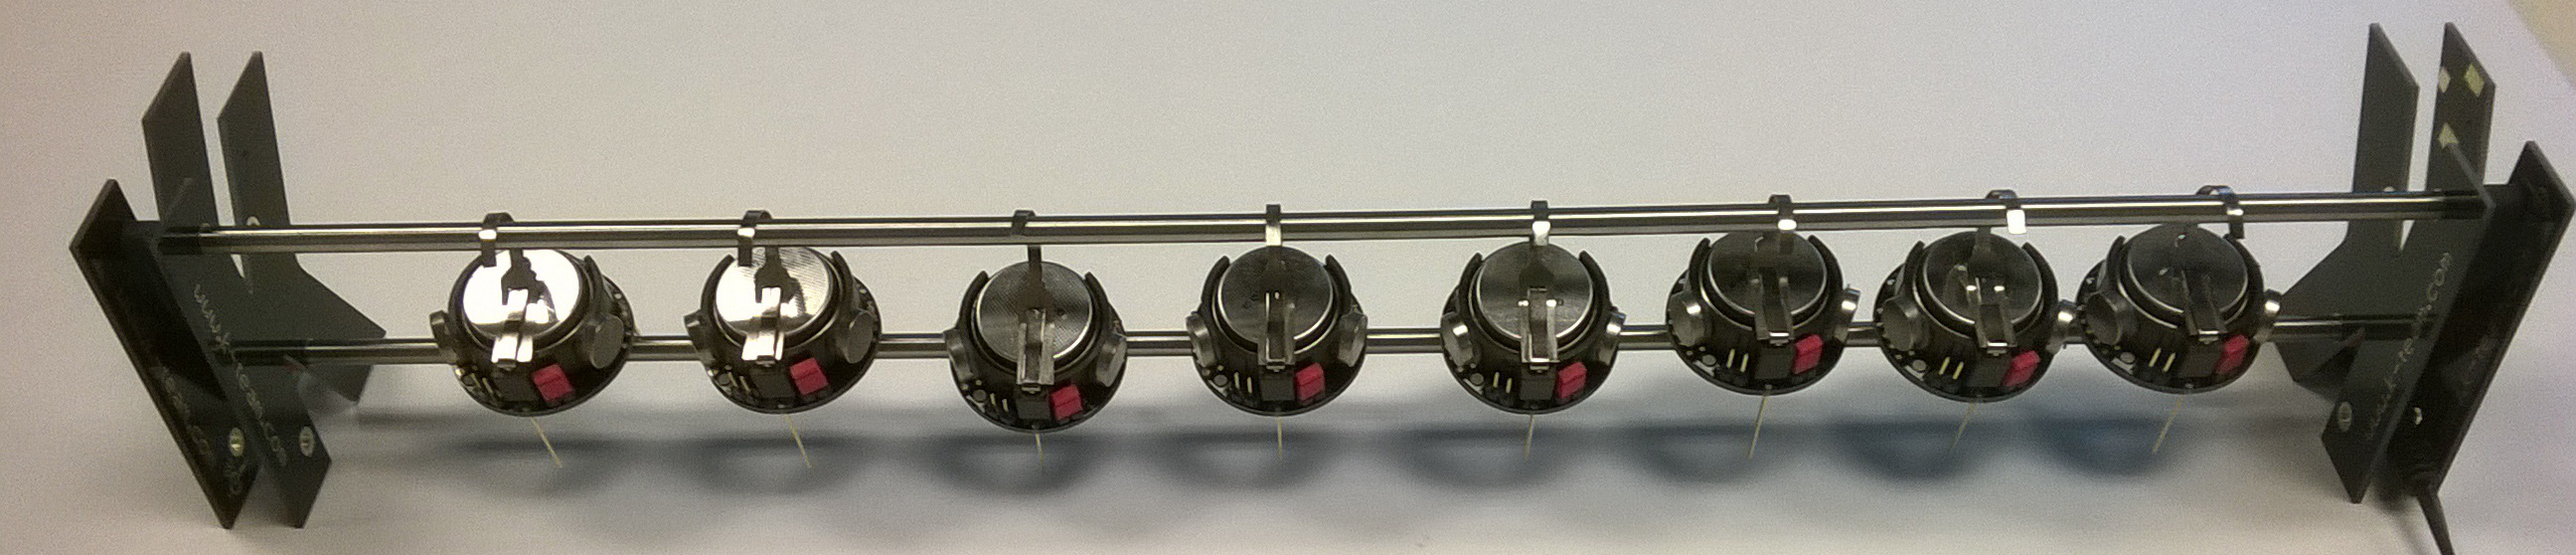
\includegraphics[width=16cm]{images/kilobots_charging.jpg}}
    \caption{Kilobots sur le chargeur}
\end{figure}


\begin{center}
  \fcolorbox{red}{white}{
    \begin{minipage}{1.0\textwidth}
      Attention, en fonction de la version de kilogui dont vous disposez, il se peut que vous ne disposiez pas du bouton charge. Il existe deux versions de kilogui: La version sous format .deb contient la calibration mais pas le mode charge. Il faut donc r\'ecup\'erer les sources de kilogui et les compiler vous-même.\\
      Attention, les sources de kilogui ne contiennent pas la calibration. Il faut donc utiliser les deux versions en fonction de l'action souhait\'ee (calibration ou chargement).
    \end{minipage}
  }
\end{center}

\subsection*{Compilation d'un programme pour les kilobots}\label{sec:name}
\addcontentsline{toc}{subsection}{Compilation d'un programme pour les kilobots}

Pour compiler un programme pour la plate-forme Kilobot, il suffit de changer dans le Makefile la valeur de la variable \textit{EXEC} en d\'ebut de fichier par le nom du fichier \`a compiler.\\

\begin{center}
  \fcolorbox{red}{white}{
    \begin{minipage}{1.0\textwidth}
      Attention, si la compilation \'echoue veuillez v\'erifier si les logiciels suivants sont install\'es : \textbf{avr-libc}, \textbf{gcc-avr} et \textbf{avrdude}.\\
    \end{minipage}
  }
\end{center}

\subsection*{Calibration des kilobots}\label{sec:name}
\addcontentsline{toc}{subsection}{Calibration des kilobots}

Les kilobots se déplaçant par vibration, il est primordial de les calibrer. En effet, chaque exemplaire possède des pattes avec un angle différents. Il faut donc les calibrer individuellement.
Pour calibrer un robot, allumer le puis positionner le en dessous du contrôleur. Vérifier que vous utilisé bien la version de kilogui disposant du module de calibration (la 64 bits).\\
Cliquer sur le bouton de calibration, vous obtenez la fenêtre suivante :

\begin{figure}[!h]
    \centering
    \subfigure{ 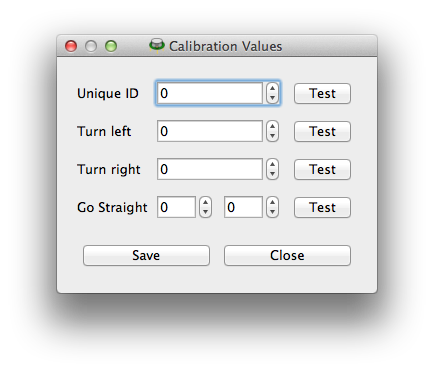
\includegraphics[width=10cm]{images/calib.png}}
    \caption{Interface de calibration de KiloGUI}
\end{figure}

Elle comporte 5 champs :

\begin{description}
\item[Unique ID] : permet d'associer à chaque kilobot un identifiant.
\item[Turn Left] : permet de définir la puissance de vibration utilisé par le kilobot pour tourner à gauche. Ce sera la valeur utilisé par la constante kilo\_turn\_left. Une puissance entre 60 et 90 est généralement suffisante pour obtenir une bonne rotation. Cliquer sur Test pour tester la nouvelle valeur.
\item[Turn Right] : idem que Turn Right. Attention : il a de grande chance qu'il faille utiliser une valeur différente que celle utilisé pour Turn Left.
\item[Go Straight] : Valeur utilisé par le kilobot lorsqu'il désire avancer en ligne droite. Chaque valeur correspond à un moteur de vibration. Une fois encore, il est fort probable que les valeurs requises soient différentes des valeurs précédentes.
\end{description}

Une fois la calibration terminée, cliquer sur Save pour enregistrer les nouvelles valeurs dans la mémoire du kilobot.

\newpage
\section*{Codes Sources}\label{sec:name}
\addcontentsline{toc}{section}{Codes Sources}

\subsection*{Luciole/Firefly}\label{sec:name}
\addcontentsline{toc}{subsection}{Luciole/Firefly}
\lstinputlisting[language=C]{../src/firefly.c}

\newpage
\subsection*{Orbit : maitre}\label{sec:name}
\addcontentsline{toc}{subsection}{Orbit : maitre}
\lstinputlisting[language=C]{../src/orbit_master.c}

\newpage
\subsection*{Orbit : esclave}\label{sec:name}
\addcontentsline{toc}{subsection}{Orbit : esclave}
\lstinputlisting[language=C]{../src/orbit_slave.c}

\newpage
\subsection*{Phototaxis}\label{sec:name}
\addcontentsline{toc}{subsection}{Phototaxis}
\lstinputlisting[language=C]{../src/phototaxis.c}

\newpage
\subsection*{Gradient}\label{sec:name}
\addcontentsline{toc}{subsection}{Gradient}
\lstinputlisting[language=C]{../src/gradient.c}

%%%%%%%%%%%%%%%%%%%%%%%%%%%%%%%%%%%%%%%%%%%%%%%%%%%%%%%%%%%%%%%%%%
%                                                                %
%                          BIBLIOGRAPHIE                         %
%                                                                %
%%%%%%%%%%%%%%%%%%%%%%%%%%%%%%%%%%%%%%%%%%%%%%%%%%%%%%%%%%%%%%%%%%
\nocite{*}
\bibliographystyle{plain}
\bibliography{kilobot}
%\addcontentsline{toc}{chapter}{Bibliographie}

\end{document}
